\documentclass{scrartcl}
\usepackage{tikz}
\usetikzlibrary{arrows,automata}
\usepackage{comment}
\begin{document}
\hfuzz=\maxdimen
\tolerance=10000
\hbadness=10000
\begin{center}
Wen Liang(\texttt{Wen\_Liang@student.uml.edu}) 01724877
\end{center}



\noindent$\textbf{0.1}$
\\

 \noindent$a.\,\,$including all the positive odd numbers\\
 $b.\,\,$including all the even numbers\\
 $c.\,\,$including all the positive even numbers and 0\\
$d.$\,\,including all the positive even numbers, 0, and multiple of 3\\
 $f.\,\,$w is a string consists of 0 and 1, if we reverse the string w, we can still get the same w\\
  $e.\,\,$this set is empty set $\phi$, because we can not find the integer has this kind of property\\
\\
\\
$\textbf{0.2}$
\\
\\
$
$a.$ \,\,\{1,10,100\}\\
$b.$ \,\,\{$n$\mid$n$ \in $N$ \,and \, $n$\, > $5$\}\\
$c.$ \,\,\{$n$\mid$n$ \in $N$ \,and \, $n$\, < $5$\}\\
$d.$ \,\,\{``aba"\}\\
$e.$ \,\,\{\epsilon\}\\
$f.$ \,\,\phi\\
$ 
\\
\\
$\textbf{0.3}$
\\
\\
$a.\,\,$No\\
$b.\,\,$Yes\\
$c.\,\,$\{x,y,z\}\\
$d.\,\,$\{x,y\}\\
$e.\,\,$\{(x,x),(x,y),(y,x),(y,y),(z,x),(z,y)\}\\
$f.\,\,$\{$\phi$,\{x\},\{y\},\{x,y\}\}\\
\\
\\

\noindent$\textbf{0.4}$
\\
\\
ab, because each element in A pair with each element in B, so we have ab elements in total
\\
\\
$\textbf{0.5}$ 
\\
\\
$2^c$ , consider each subset consist of 1 elements, 2 elements, 3 elements,..., c elements. So we have $C_c^1+C_c^2+C_c^3+...+C_c^c=2^c$\\
\\

\noindent$\textbf{0.6}$
\\
\\
$a.\,\,$7\\
$b.\,\,$domain:\{1,2,3,4,5\}\,\,\,\,\,range:\{6,7\}\\
$c.\,\,$6\\
$d.\,\,$domain:\{(1,6),(1,7),(1,8),(1,9),(1,10),(2,6),(2,7),(2,8),(2,9),(2,10),\\
(3,6),(3,7),(3,8),(3,9),(3,10),(4,6),(4,7),(4,8),(4,9),(4,10),(5,6),(5,7),(5,8),(5,9),(5,10)\}\\
\indent{}range:\{6,7,8,9,10\}\\
$e.\,\,$8\\
\\
\\
$\textbf{0.7}$
\\
\\
Let A=\{1,2,3,4\}\\ \\
$a.$ The relation R = \{(1,1),(2,2),(3,3),(4,4),(2,1),(1,2),(3,2),(2,3)\} is reflexive and symmetric, but not transitive, because(1,2) $\in$ R and (2,3) $\in$ R but (1,3) $\notin$ R. \\
$b.$ The relation R = \{(1,1),(2,2),(3,3),(4,4),(1,2)\}is reflexive
and transitive, but not symmetric because (1,2)$\in$ R but(2,1) $\notin$ R\\
$c.$ The relation R =\{(1,1),(2,2),(3,3)\} is symmetric and transitive, but not reflexive, because 4 $\in$ A but (4,4) $\notin$ R. \\

\noindent$\textbf{0.8}$
\\
\\
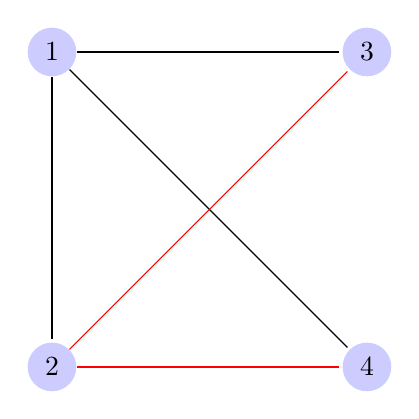
\begin{tikzpicture}[>=stealth',shorten >=1pt,auto,node distance=4cm,every node/.style={circle,fill=blue!20}]
\node 	(1)      				{$1$};
 \node 	  (2) [below of=1]  	{$2$};
  \node  	(3) [right of=1]  	{$3$};
	\node   (4) [right of=2]   {$4$};
	
	\path[-] (1)  edge  	 	(2)
             edge           	(3)
						edge	(4)
        (2) edge[color=red]  		 	(3)
             edge[color=red] 			 	(4);
        
\end{tikzpicture}

\begin{center}
 \begin{tabular}{||c c ||}
 \hline
  node 	& degree		\\ [0.5ex] 
 \hline
 $1$ 		& 3	\\
 \hline
 $3$ 		& 2	\\
 \hline
\end{tabular}
\end{center}

Path: 3 $\to$ 2 $\to$ 4
\\
\\
$\noindent\textbf{0.9}$
\\
\\
$(\{1,2,3,4,5,6\},\{(1,4),(1,5),(1,6),(2,4),(2,5),(2,6),(3,4),(3,5),(3,6)\})$
\end{document}




















